\documentclass{article}
\usepackage{url}
\usepackage{graphicx}
\graphicspath{{./images}}
\title{Malware Reverse Engineering \\
Practical 2 Report \\
Spring 2022}
\author{Michael Ivanov \\
ivanovmichael@ufl.edu}
\date{March 14, 2022}

\begin{document}
    \maketitle
    \pagebreak
    \section{Executive Summary}
    \pagebreak
    \section{Static Analysis}

    \subsection{MD5 Hashes}
    \begin{itemize}
        \item sample2.exe: E05D85ACC62B2795BFB94A681E64E20F
        \item resource1 IDR{\_}X86BOT: 958596F72BD381520A75FFA6E4DB9827
        \item resource2 IDR{\_}X86LOADER: 27DA8F25FF1CB54C63618D2A489EE4DF
        \item resource3 IDR{\_}X86BOT: E8AF535C7447D203FF7CD44440B00459
    \end{itemize}

    \subsection{Program Compilation Date}
    \begin{itemize}
        \item sample2.exe: Fri Aug 19 09:54:32 2016
    \end{itemize}

    \subsection{Suspicious Imports}
    \begin{itemize}
        \item \textbf{CreateProcessW:} This gives an indication the malware could be creating other processes.
        \item \textbf{TerminateProcess:}
        \item \textbf{VirtualProtect:} This can be used to change the permissions and protections of a process.
        \item \textbf{NtQueryInformationProcess:} Can be used to retrieve information about a specified process.
    \end{itemize}

    \subsection{Suspicious Strings}
    \begin{itemize}
        \item \textbf{"Wow64DisableWow64FsRedirection":} A function that disables file system redirection for the calling thread.
        \item \textbf{"FindResource", "LoadResource":} Functions for finding and loading an external resource.
        \item \textbf{"Sleep":} Might be useful to know for later dynamic analysis, the program might hang for a long period of time.
        \item \textbf{".log"} A possible file extension to some kind of log file.
    \end{itemize}

    \subsection{Program sections}
    In the .rsrc (resource) section there are 3 files. I have provided the hashes above.

    \subsection{Anti-disassembly}

    \section{Dynamic Analysis}
    \subsection{Interesting behaviors}
    When the program is first executed it immediately deletes itself. However, by using Procmon I was able to see the program was still running. It was now in the \path{C:/Users/malware/AppData/Roaming} directory.
    \begin{figure}[h]
        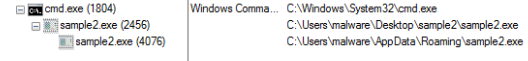
\includegraphics[width=\textwidth]{sample2process.png}
        \caption{Procmon showing the process tree of sample2.exe}
    \end{figure}
    \subsection{Contacted machines and services}
    \subsection{Registry Keys created/modified}
    Created Keys:
    \begin{itemize}
        \item \path{HKLM\System\CurrentControlSet\Services\Tcpip\Parameters}
    \end{itemize}
    \begin{figure}[h]
        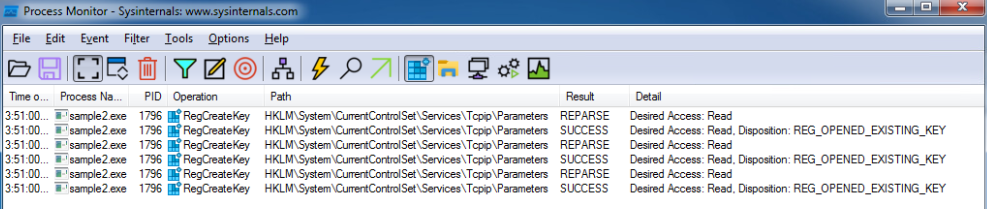
\includegraphics[width=\textwidth]{RegKeyCreate.png}
        \caption{Procmon showing the attempted creation of a registry key}
    \end{figure}
    \subsection{Files created/modified}
    Files Created:
    \begin{itemize}
        \item \path{C:\Windows\System32\imm32.dll}
        \item \path{C:\Windows\System32\sechost.dll}
        \item \path{C:\Windows\System32\winhttp.dll}
        \item \path{C:\Windows\System32\webio.dll}
        \item \path{C:\Windows\System32\IPHLPAPI.dll}
        \item \path{C:\Windows\System32\winnsi.dll}
        \item \path{C:\Windows\System32\rpcss.dll}
        \item \path{C:\Windows\System32\cryptbase.dll}
        \item \path{C:\Windows\System32\ncrypt.dll}
        \item \path{C:\Windows\System32\bcrypt.dll}
        \item \path{C:\Windows\Globaliztion\SortDefault.nls}
        \item \path{C:\Users\malware\AppData\Roaming\sample2.exe}
        \item \path{C:\Windows\System32\apphelp.dll}
        \item \path{C:\Windows\AppPatch\sysmain.sdb}
    \end{itemize}
    \subsection{Processes started}
    \subsection{Persistence}

\end{document}